\chapter{Architecture and Implementation}
\label{architecture_and_implementation}

In the previous chapter, the foundation for implementing a system that does route optimization for snow plowing has been outlined. It has been shown why the NEARP has been chosen as the underlying model. Further, it was argued why MAs are a good approach to the problem. Then issues relating to the combination of the snow plowing problem and MAs solving the NEARP were discussed.

Now with the background of our implementation sorted out, the architecture should be addressed. The main flow of the system is illustrated in Figure \ref{fig:system_flowchart}. Here we can see that the first thing to happen is that input data is converted to the NEARP format \citep{NEARPdocumentationSINTEF} for use by the MA.

\begin{wrapfigure}{o}{0.47\textwidth}
    \begin{center}
        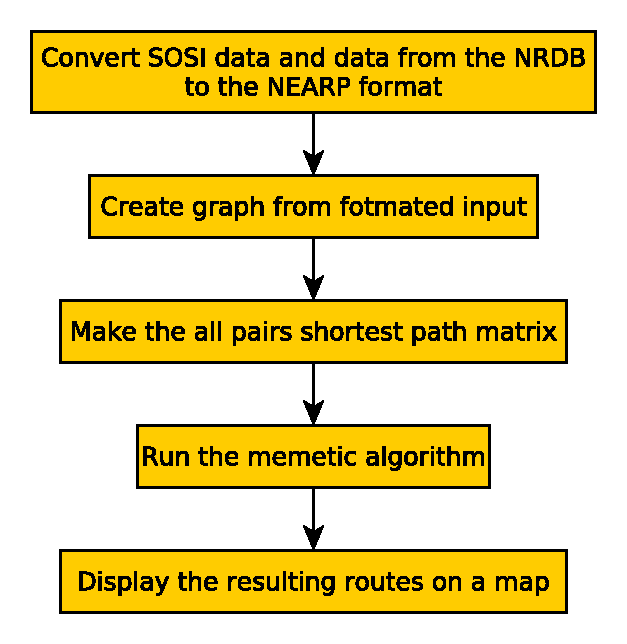
\includegraphics[width=0.46\textwidth]{figures/Architecture/Overal_system_workflow.pdf}
    \end{center}
    \caption{Overview of the systems Workflow}
    \label{fig:system_flowchart}
\end{wrapfigure}

\section{Data Sources} % (fold)
\label{sec:data_sources}

% section data_sources (end)

The data comes from two main sources. The first one is the municipality's map data, supplied in files adhering to the Norwegian SOSI-Standard for map data \citep{kartverketSOSI}. Most importantly, the maps contain information about what set of roads and intersections make up each existing route. These roads can then be used as the required elements of a route the MA is supposed to optimize the servicing of. The sets of roads can also be utilized for evaluating how the drivers currently drive their routes with the fitness function used by the MA. This fitness can then be used to evaluate how good the results of the MA are by comparing it to the best fitness the MA finds for the same set of roads.

Another important piece of data that the municipality's maps contains are modifications to the infrastructure made by and maintained by the municipality. The most important example would be barriers. As shown in Figure \ref{fig:environmental_factors} some of the barriers can be passed by snow plowing vehicles, while other barriers can not. The municipality's maps detail which can and which can not be passed.

What other information about the infrastructure that is required but not contained in the municipality's data set can be found in the NPRAs data. Their database of roads, the NRDB, contains highly detailed information about the road network. It covers physical features such as length, width, and curvature, as well as meta-information such as speed limits, placement of signs, and where pedestrian crossings are located.

\section{Formatting Input and Output} % (fold)
\label{sec:achitecture_formatting_input_and_output}

The process of making an input file based on all this data is done in the following way. First the road networks from the municipality's maps and the NRDB are combined into a single dataset with PostGIS. The combination relies on matching the geometries of items in the maps, combining items into a new one if they are within a certain distance of each other, otherwise copying them in. For most parts, this worked well, but there were some roads and required elements that go missing in the process. One reason for the missing pieces is how the merging of the municipality's data and the NRDB data is done. Because the merging is done by combining elements closer than five meters apart in the data into one it sometimes merges roads that should have been separate. The missing pieces are however easily found on inspection and drawn in. Nevertheless there might be errors in the data set used further that have not been discovered at the time of writing.

\begin{wrapfigure}{o}{0.5\textwidth}
    \begin{center}
        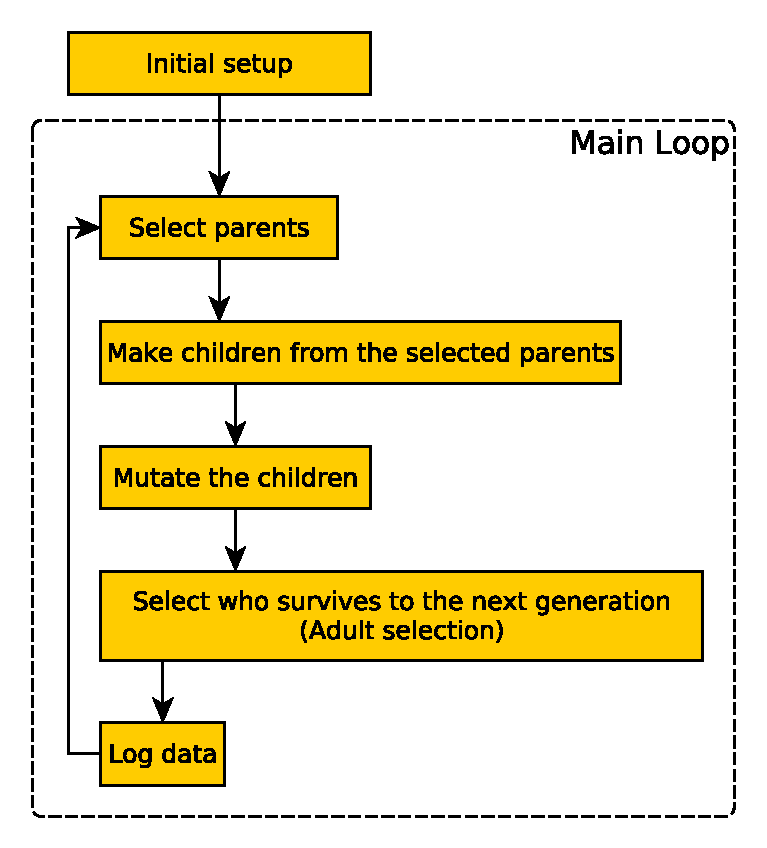
\includegraphics[width=0.5\textwidth]{figures/Architecture/MA_flowchart.pdf}
    \end{center}
    \caption{Memetic Algorithm Flowchart}
    \label{fig:ma_flowchart}
\end{wrapfigure}

This set is then converted into a graph with nodes, edges, and arcs. The intersections become nodes, and the ones that are part of a route in the municipality's maps are labeled as required. One-way streets are converted to arcs and other roads to edges. When working with routes for car roads, bicycle paths, pavements, and sidewalks are ignored. The main reason for ignoring them is because they in most cases cannot be utilized by the vehicle's operation on the car roads for passing through. Also when finding routes for plowing car roads they do not have to be considered for servicing.

However, even though the other types of roads do not have to be serviced, in some cases they should be considered wile servicing the car roads. For instance, when a sidewalk and adjacent car road are both plowed the order matters. When the road is plowed snow is going to move to the side and onto the sidewalk. Therefore, if each of the routes are to be driven only once the road should be serviced first, then the sidewalk. With that ordering the snow will move off the road to the sidewalk and then off the sidewalk. Otherwise the sidewalk would just end up filled with snow again after it has been cleared. It is however chosen to ignore the interaction between servicing adjacent routes in this work. The reasoning behind doing so is that it simplifies the model and allows for working on each route individually.

When making arcs and edges, the ones that are part of a route are labeled as required, just like the nodes. The arcs and edges are then assigned a traversal cost, that describes how much resources are spent passing through them without performing work on them. For car roads, this is set to be: $\text{Traversal cost} = len \times (150 - lim)$. In the equation $len$ is the length of the road described by the arc or edge, and $lim$ is the speed limit on the stretch. For other kinds of underlying roads or paths, the traversal cost is set to just the length. Subtracting the speed limit from 150 before multiplying is done so that faster roads get priority due to that the fitness is considered better when lower.

After the traversal costs are determined for the arcs and edges, the required elements get their demands and servicing costs set. The demand of each element, in the case of snow plowing representing the amount of snow that each vehicle should handle the removal of, is set to be the length of the element. The same is done for the servicing cost. The main reason for choosing the length for these values is that the length scales with the amount of work that needs to be done, and resources needed to carry out the work. Additionally the servicing cost amounts to the same for each trip matter what order it is processed in, so it will not affect the fitness of the individuals.

This process for converting to and from the NEARP format for the MA has been designed in collaboration with Magnus Solheim Thrap and Christoffer Viken. We all took part in deciding how the data should be mapped to the NEARP format. Thrap found how to extract certain features from the data in the NRDB. Viken has been able to combine the data from the NRDB and the municipality in PostGIS. Then the omissions from the conversion are remedied in PostGIS, exported as CSV files and converted to the NEARP format with a script written in Python. Finally, the resulting routes are converted back to CSV, and Viken has found a way to draw them on a map using PostGIS.

% section formatting_input_and_output (end)

\section{Memetic Algorithm Implementation} % (fold)
\label{sec:memetic_algorithm_implementation}

Now when the implementation of how the MA takes input has been outlined, the architecture of the MA itself can be discussed. The workflow in the MA is shown in Figure \ref{fig:ma_flowchart}. From the figure, it can observed that the first step is generating an initial population. This population is either generated completely at random, or seeded from known routes. The seeding can be done for instance when working with existing routes, to see whether the MA can improve on them, or if routes with better fitness can be generated faster.

\subsection{Parent Selection} % (fold)
\label{sub:achitecture_parent_selection}

Once the initial population has been generated, the MA enters its main loop. Here it will first select which individuals get to breed in the parent selection. In our implementation, there are three possible ways of doing the parent selection. Uniform selection, fitness proportionate selection, and tournament selection. All the parent selections are implemented with replacement, but with the constraint that no pair of parents can have two equal individuals. That is, one individual can have several mates each generation, but cannot mate with itself.

If using uniform selection, the parents are selected completely at random from the adult population, i.e., they have a uniform probability of being selected. The fitness proportionate selection is biased towards picking individuals with better fitness for being parents, by giving each individual a probability of being chosen that is $P(\text{selecting individual}) = \frac{\text{the fitness of the individual}}{\text{sum of fitnesses of all adult individuals}}$.

Tournament selection picks individuals for parenthood by making groups of individuals it selects from. For each parent it selects, it creates a group of fixed size that is determined by the operator on startup, which is sorted by fitness. Then, with a chosen probability $P$ it selects the best individual. Should the best individual not be selected, it goes on to the second best and determines whether to select it with the same probability $P$. The tournament with the individuals stacked against each other continues until a parent is selected, or all individuals other than the worst in the group have failed. In the event that all better individuals in the group fail to be selected, the worst one is selected. This gives the best individual a probability of $P$ of being selected, the worst one $(1-P)^{\text{tournament group size}-1}$, and the ones in between $(1-P)^{n} \times P$, where $n$ is the number of better individuals in the tournament group.

% section parent_selection (end)

\subsection{Child Creation} % (fold)
\label{sub:achitecture_child_creation}

When the parent selection has been done, the selected pairs of parents are used for generating children with the crossover procedure, which is illustrated in Figure \ref{fig:crossover_illustration}. The crossover works by first selecting two random crossover points. Then, for each parent, every element in the genome that is between these points is copied to a child genome. The rest of the child genome that is not between the crossover points is then filled with the remaining required elements. They are inserted in the same order as they appear in the other parent after the second crossover point. This process ensures the child genomes maintain their properties as circular representations of all the required elements from the graph, and that they inherit traits from both parents.

\begin{figure}[thbp]
    \centerline{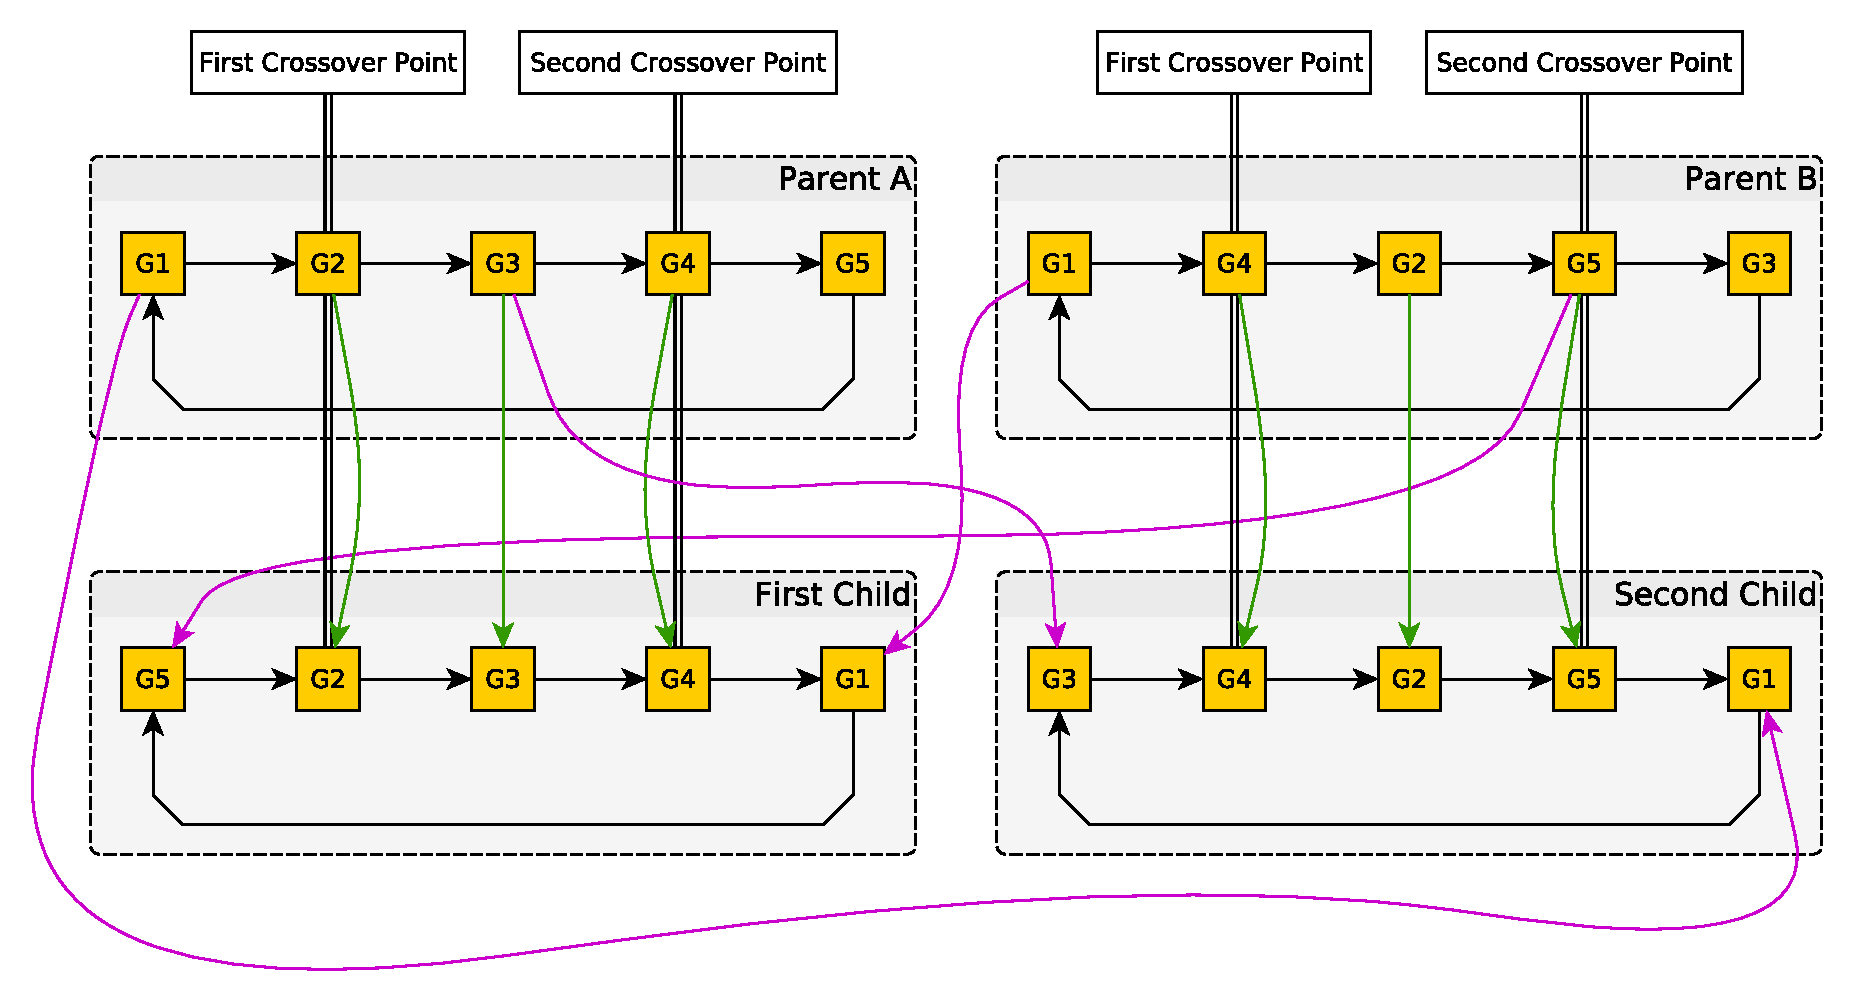
\includegraphics[width=\textwidth]{figures/Architecture/Crossover_Illustration.pdf}}
    \caption{Crossover with two parents and two crossover points}
    \label{fig:crossover_illustration}
\end{figure}

After all the children have been generated, the MA mutates them. In our implementation, this step is done by either swapping two elements in their genomes at random or performing a memetic improvement of the genomes. The memetic improvement is done by swapping two and two elements in the genome, and evaluating the fitness of the outcome. This process is repeated until the swap results in an improvement fitness, or all swaps have been tried.

% subsection child_creation (end)
\subsection{Adult Selection} % (fold)
\label{sub:achitecture_adult_selection}

Then, when the children have been made and mutated, the adult selection is performed. It is the process where one determines what individuals from the adult population and children are kept and used as adults in the next generation. There are four kinds of adult selection methods in our implementation, full replacement, elitist mixing, random mixing, and overproduction. With full replacement, there are made exactly as many children as the size of the population is at the start of each generation. In the transition, all the previous individuals are discarded, and the children become the new population.

If doing elitist mixing, the number of children can be arbitrarily chosen. When going to the next generation, the children and adults are combined into one large pool. Then the ones with the best fitnesses get the slots in the new population, and all the other are discarded. Random mixing works much in the same way as elitist mixing, except that the individuals are chosen from the pool at random, instead of by fitness. The approach when using overproduction is to create more children than there are individuals at the start of the next generation. In the transition to the next generation, the best children are used, and the rest of the old generation is discarded.

% subsection adult_selection (end)

\subsection{Generation Transition} % (fold)
\label{sub:achitecture_generation_transition}

% section generation_transition_s (end)

After the adult selection has been done, the worst individual of the new generation is removed, and the previous best is inserted in its place. Then the halting conditions for the MA are checked, and if they are met the algorithm terminates. Of the two conditions that are checked for, the first one is whether there have been no improvements in the best individual found for a number of generations which is determined on startup. The second is whether a fixed number of generations has elapsed since the MA was started. Once it has terminated, the output can be drawn on a map.

% section memetic_algorithm_implementation (end)

\cleardoublepage
